%----------------------------------------------------------------------------
\chapter{Teljesítményelemzés és optimalizálás}
%----------------------------------------------------------------------------

(3-4 oldal)

Derp derp, valami szöveg. Árvíztűrő tükörfúrógép.

Selenium tesztek


%----------------------------------------------------------------------------
\section{Kollaborációs teljesítményelemzés}
%----------------------------------------------------------------------------


%----------------------------------------------------------------------------
\subsection{Szimuláció}
%----------------------------------------------------------------------------
A szimuláció célja automatizálni a felhasználói bemenetet egy teljesítmény méréshez. A megoldásnak tartalmaznia kell alapszintű felhasználói bemenet szimulálását: egérkattintás, szövegbeírás, várakozás és mivel egy grafikus modellt akarunk szerkeszteni a ``drag and drop'' funkcióra is szükség van. 

A böngészőautomatizálás Selenium Webdriver segítségével történt, ez az eszköz lehetővé teszi, hogy különböző nyelveken megírt (Python, Java, PHP stb. ) teszt esetekben a Webdriver API-val kommunikálva böngésző példányokat lehet irányítani. 
Seleniumhoz tartozik egy grafikus fejlesztőkörnyezet is ami Selenium IDE néven Firefox böngészőkiegészítésként fut, vele rögzíteni lehet felhasználói bemenetet és egér eseményeket, majd egy ilyen felvételt újralejátszani, módosítani. Ez előnyös teszterek számára akik repetitív munkát végeznek és nem tudnak programozni, de fejlesztők számára is jó, mert ezekből a felvételeket Python, Ruby stb teszteseteket lehet exportálni. 
Azon kívül, hogy automatizált tesztelésre a szkriptek alkalmasabbak, a Selenium IDE sajnos nem tud egérmozgatást rögzíteni, így nem hasznos a feladat szempontjából. A Selenium API javascript implementációját példáúl a selenium-webdriver csomag valósítja meg, viszont hamarosan kiderült, hogy ez a csomag nem támogatja ``drag and drop'' funckciót, emiatt a Python implementációt választottam. 

A fejlesztés korábbi stádiumában meg kellett győződni, hogy az alkalmazás valamennyire tűri a rossz internetkapcsolatot, ezért egy teszt környezetet alakítottam ki amiben két felhasználót szimulálva két selenium szkript ugyanazt a dokumentumot szerkeszti és véletlenszerű változtatásokat hajt végre a diagramon, pontosabban véletlen entitást mozgat el véletlen irányba. Az elvárt eredmény az, hogy rossz internet kapcsolat mellett is sok idő elteltével ugyanazt a diagramot látja a két felhasználó és azt, hogy ``ugyanazt'' a diagramot látják a diagram hash megegyezése igazolja.
 

\begin{figure}[!ht]
\centering
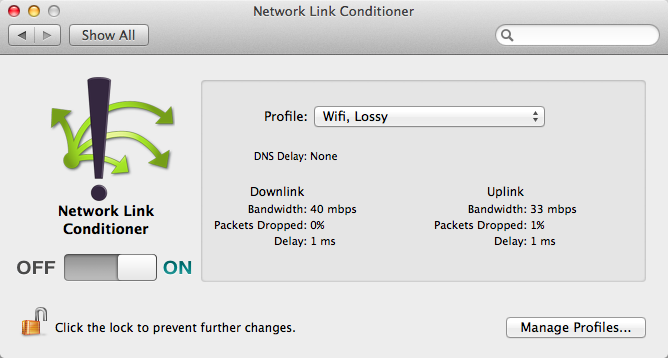
\includegraphics[width=15cm,keepaspectratio]{figures/nlc.png}
\caption{OSX Network Link Conditioner}
\label{fig:nlc}
\end{figure}


A rossz internet kapcsolat szimulálásához OSX-en a Network Link Conditioner alkalmazást használtam, ami az XCode fejlesztőkörnyezet egy kiterjesztése. A felhasználói felülete elég egyszerű és maximálisan megfelel a funkcionalitása a szimulációhoz, ezen kívül a létező profilok is hasznosak, ha példáúl egy gyenge jelű 3G kapcsolatot akarunk szimulálni. A paraméter amire kiváncsi voltam az a csomagvesztési arány volt, úgy azt kezdtem állítani egyre magasabb értékre. Az eszköz bekapcsolása után a ping parancssoros eszköz segítségével egy publikus ip-t pingelve\footnote{példáúl \lstinline{ping www.google.com}} kipróbáltam, hogy valóban akkora a csomagvesztés.

Az eredmény meglepő volt: már olyan csomagvesztési aránynál, ami nekem kicsinek tűnt, példáúl 10-20\% ?????nem lehetett bongeszni????
de a diagram egyezett a két felhasználónak. Wireshark protokolanalizátor segítségével megvizsgáltam, hogy ez miért is lehet, hogy nem veszett el esemény:


\begin{figure}[!ht]
\centering
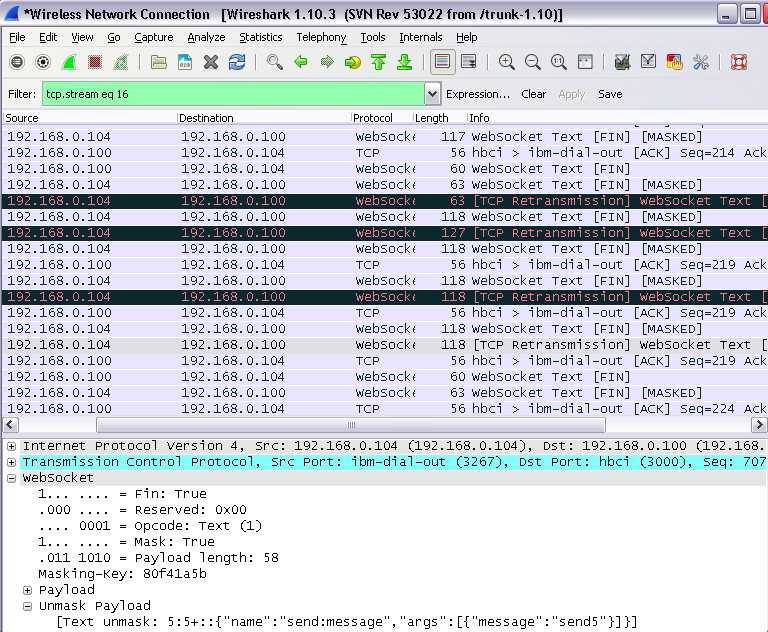
\includegraphics[width=15cm,keepaspectratio]{figures/wireshark.png}
\caption{A Websockets forgalom vizsgálata Wireshark segítségével}
\label{fig:wireshark}
\end{figure}


Wireshark-ban a Websockets protokoll-ra filtereltem, és egy újraküldött csomagra kattintva (a fekete sorok egyike) megnéztem az adott TCP folyamot. Látszik, hogy 192.168.0.104 -- a kliens ebben az esetben -- websockets üzeneteket küld, és a szerver TCP nyugtát küld (ACK) és amikor ez nem történik meg, akkor újraküldődik az üzenet.



++++++++++++++++++++++++
random módon két ember crudol és le kell mérni , hogy mennyire valószínű, hogy elvésznek a bemenetei
++++++++++++++++++++++++

%----------------------------------------------------------------------------
\section{Kliens oldali teljesítményelemzés}
%----------------------------------------------------------------------------
Derp.

%----------------------------------------------------------------------------
\section{Webszerver teljesítményelemzés}
%----------------------------------------------------------------------------
Derp.

%----------------------------------------------------------------------------
\section{Adatbázis teljesítményelemzés}
%----------------------------------------------------------------------------
Derp.





